%seminarska naloga
\documentclass[seminar, slovene]{FRIreport}

% AMS fonts required
\usepackage{iopams}  

% package to include graphics in ps, eps or png format
\usepackage{graphicx}
\usepackage{epstopdf}
% the graphics path
\graphicspath{{img/}}

% define equation referencing
\newcommand{\eqref}[1]{(\ref{#1})}

% define figure referencing
\newcommand{\figref}[1]{\ref{#1}}

% define real numbers symbol
\newcommand{\Rset}{\ensuremath{\mathbb{R}}} 
\newcommand{\R}{\Rset} 
% define natural numbers symbol
\newcommand{\Nset}{\ensuremath{\mathbb{N}}} 
\newcommand{\N}{\Nset} 
% define euclidean vector space symbol
\newcommand{\Eset}{\ensuremath{\mathbb{E}}} 
\newcommand{\E}{\Eset} 

\newcommand{\imp}[1]{{\color{P654M}#1\normalcolor}}

%%%
\newcommand{\angl}[1]{(\textit{angl.} #1)}

%main
\begin{document}

\title{QCA sekven\v cna ALE}

\author{Miha Zidar, Anže Pečar, Matic Potočnik, Željko Plesac, Jan Varljen}

%\address{Skupina 1}

\begin{abstract}
V seminarski nalogi bomo opisali zasnovo sekvenčne ALE s kvantnimi celičnimi avtomati, z uporabo programa QCAdesigner.

\Keywords{kvantni celični avtomati, aritmetično-logična enota, modeliranje in simulacija}
\end{abstract}

%
%%
\section{Uvod}
\subsection{Ideja}
V tej seminarski nalogi bomo opisali zasnovo sekvenčne ALE s kvantnimi celičnimi avtomati \angl{quantum cellular automata -- QCA}. Modelirali jo bomo z uporabo odprtokodnega programa QCADesigner\cite{walus:2004}, za skice logičnih vezij, pa bomo uporabili TinyCAD.
\ \\ \ \\
Sekvenčnost enote tu pomeni, da enota ne izvaja operacij nad vsebino končno dolgih registrov, ampak sprejema tok bitov, nad posameznimi biti izvaja operacije in tudi svoj izhod podaja kot tok bitov. Za določene operacije tak pristop ni praktičen, ali pa je celo nemogoč, je pa mogoče na tak način implementirati poln funkcijski sistem, kar smo v nalogi tudi storili.

\subsection{Motivacija}
Predvideva se, da bo že čez nekaj desetletij minituarizacija in zmogljivost čipov, grajenih na siliciju, dosegla končno stopnjo in bo potrebno za večjo procesno moč preiti na drug osnovni material in najverjetneje tudi spremeniti pristop k modeliranju vezij. Ena izmed obetajočih alternativ so kvantni celični avtomati, ki obljubljajo mnoge prednosti pred klasičinimi vezji:
\begin{itemize}
\item Možnost večnivojskih vezij
\item Možnost križanja vodil
\item Enostavna realizacija nekaterih časovnih vezij
\item Potencialno nižja poraba in višji takt delovanja
\item $\dots$
\end{itemize}

%
%%
\section{Metode}
V tem odseku bomo predstavili nekatere osnovne ideje in odločitve, ki smo jih nato uporabili pri realizaciji naše ALE.

\subsection{Opis naloge}
Realizirali bomo sekvenčno ALE, s funkcijsko polnim sistemom operacij. Za izbiro operacije bomo uporabili dva bita, enota pa bo podpirala naslednje operacije:\\
\begin{table}[h!]
\begin{center}
\begin{tabular}{ | c | c | c | }\hline
\textbf{Operacija} & \textbf{Oznaka} & \textbf{Op. koda} \\ \hline
NOT & $\lnot$ & 0\,0 \\
AND & $\wedge$ & 0\,1 \\
ADD & $\oplus$ & 1\,0 \\
SUB & $\ominus$ & 1\,1 \\ \hline
\end{tabular}
\end{center}
\caption{Seznam operacij}
\label{optable}
\end{table}
\subsection{Ideje za realizacijo}
Operaciji NOT in AND sta že v osnovi bitni operaciji in je tako sekvenčna realizacija popolnoma naravna. Pri ADD tudi ni posebnih zapletov, pri SUB pa smo poskušali operirati, kot bi imeli števili zapisani v predstavitvi z dvojnim komplementom.

%
%%
\section{Rezultati}
V tem delu seminarske naloge bomo predstavili realizacijo posameznih delov ALE.
\subsection{Izbira operacije}
Izbira operacije je realizirana z dvo-bitnim demultiplekserjem, ki izbira med operacijami NOT, AND, ADD in SUB, kot smo to zapisali v \autoref{optable}.
\begin{figure}[htb]
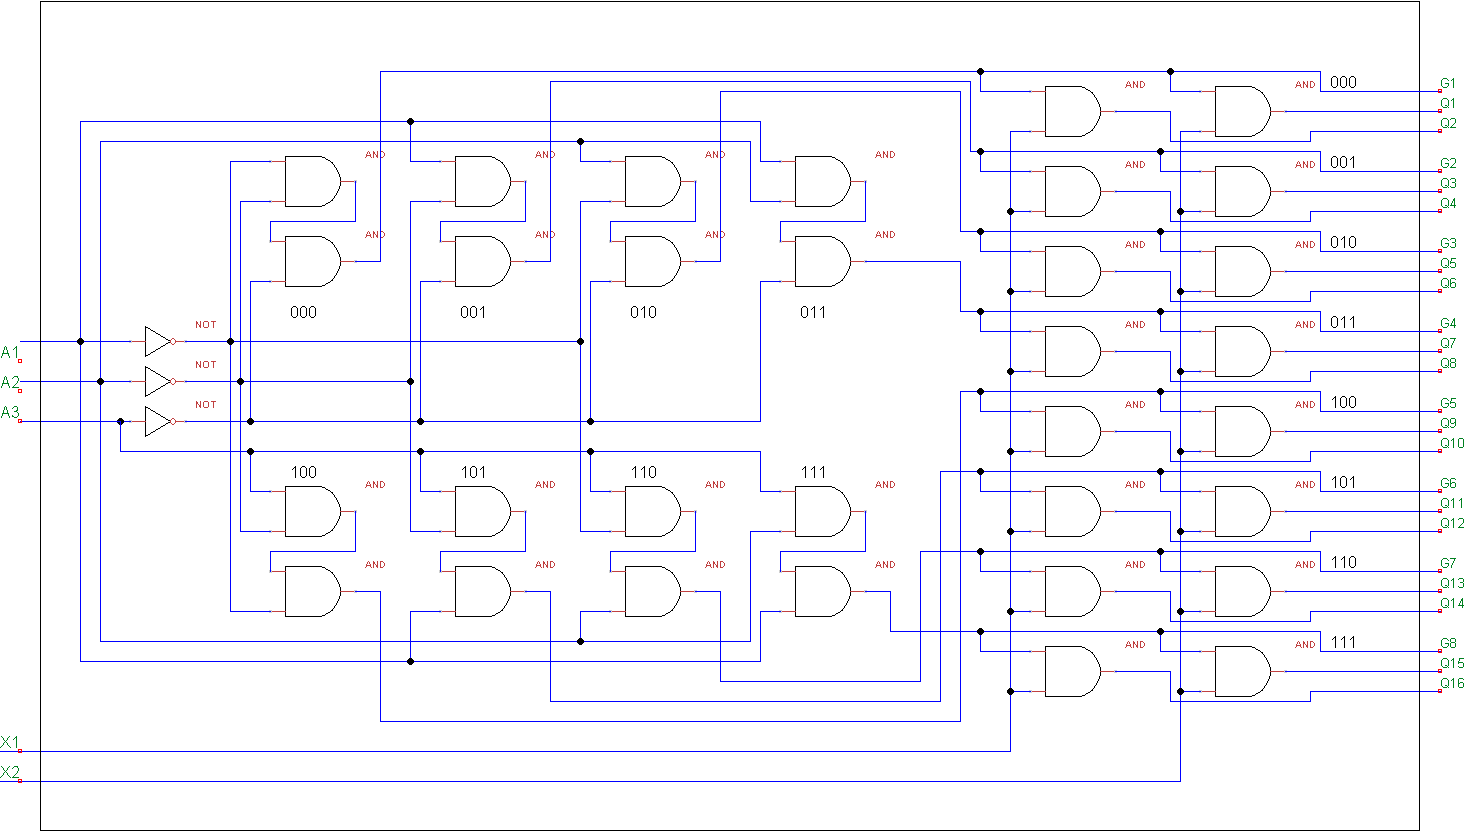
\includegraphics[width=15cm]{vezja/img/demux}
\caption{Demultiplekser}
\label{demux}
\end{figure}
\pagebreak

\subsection{Negacija}
Negacijo (operacijo NOT) smo realizirali s polovičnim zamikom celice.
\begin{figure}[htb]
\begin{center}
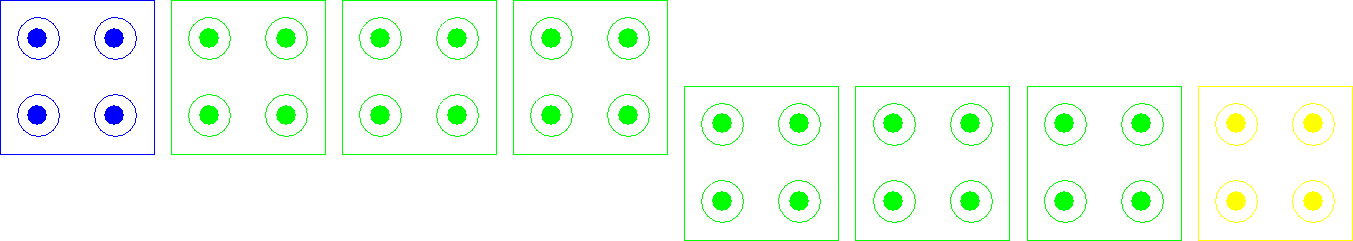
\includegraphics[width=8cm]{qca/img/NOT}
\caption{NOT vrata}
\label{NOT}
\end{center}
\end{figure}

\subsection{Konjunkcija}
Konjunkcijo (operacijo AND) smo realizirali z majoritetnimi vrati, ki imajo enega izmed vhodov nastavljenega na polarizacijo -1.
\begin{figure}[htb]
\begin{center}
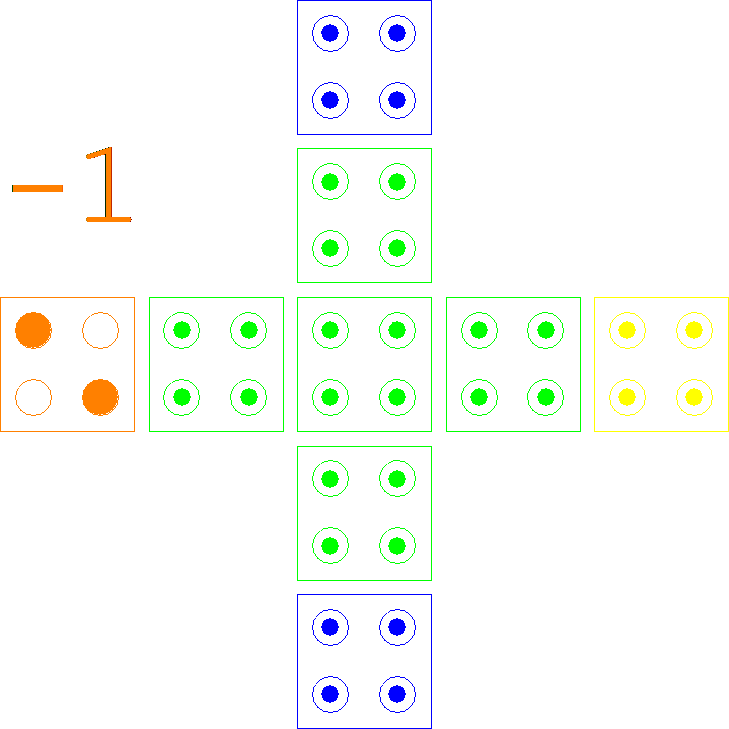
\includegraphics[width=5cm]{qca/img/AND}
\caption{AND vrata}
\label{AND}
\end{center}
\end{figure}

\subsection{Seštevalnik/odštevalnik}
Seštevalnik in odštevalnik (operaciji ADD in SUB), smo realizirali skupaj - pri odštevanju drugo število negiramo in mu pri prvem bitu prištejemo 1, kot da bi bilo zapisano v predstavitvi z dvojnim komplementom.
\begin{figure}[htb]
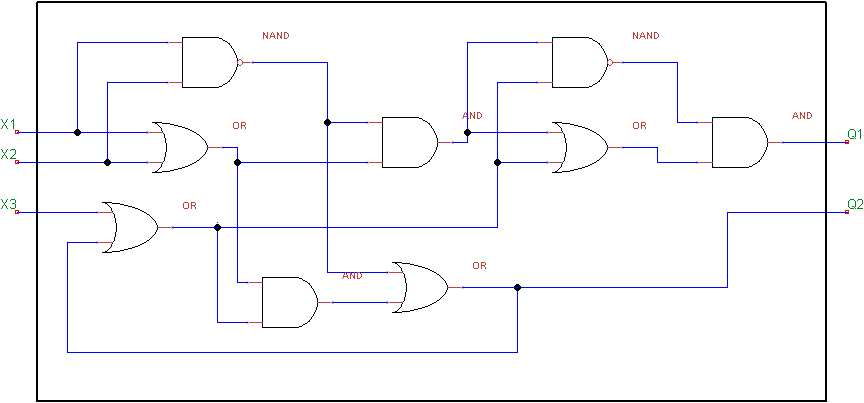
\includegraphics[width=14cm]{vezja/img/sestevalnik}
\caption{Seštevalnik}
\label{sestevalnik}
\end{figure}
\pagebreak

%
%%
\section{Zaključek}
Zaključki z nekaj izhodišči za nadaljnje delo.

%
%%
\References
\bibliographystyle{elsart-num-sl}
\bibliography{sample}

\end{document}
